\documentclass[a4paper,11pt]{article}
\usepackage{amsmath}
\usepackage{graphicx}
\usepackage{float}
\usepackage{url}

\usepackage{listings}
\usepackage{color}

\definecolor{mygreen}{rgb}{0,0.6,0}
\definecolor{mygray}{rgb}{0.5,0.5,0.5}
\definecolor{mymauve}{rgb}{0.58,0,0.82}

\lstdefinelanguage{pseudo}
{
  morekeywords={set,mod,div, if, else, end, to, foreach, then, loop},
  sensitive=false,
  morecomment=[l]{//},
  morecomment=[s]{/*}{*/},
}

\lstset {
 backgroundcolor=\color{white},   % choose the background color; you must add \usepackage{color} or \usepackage{xcolor}
  basicstyle=\footnotesize\ttfamily,        % the size of the fonts that are used for the code
  breakatwhitespace=false,         % sets if automatic breaks should only happen at whitespace
  breaklines=true,                 % sets automatic line breaking
  captionpos=b,                    % sets the caption-position to bottom
  commentstyle=\color{mygreen},    % comment style
  keepspaces=true,                 % keeps spaces in text, useful for keeping indentation of code (possibly needs columns=flexible)
  keywordstyle=\bfseries\color{blue}, % keyword style
  language=pseudo,                 % the language of the code
  numbers=left,                    % where to put the line-numbers; possible values are (none, left, right)
  numbersep=5pt,                   % how far the line-numbers are from the code
  numberstyle=\tiny\color{mygray}, % the style that is used for the line-numbers
  rulecolor=\color{black},         % if not set, the frame-color may be changed on line-breaks within not-black text (e.g. comments (green here))
  showstringspaces=false,          % underline spaces within strings only
  showtabs=false,                  % show tabs within strings adding particular underscores
  stepnumber=1,                    % the step between two line-numbers. If it's 1, each line will be numbered
  stringstyle=\color{mymauve},     % string literal style
  tabsize=2,	                   % sets default tabsize to 2 spaces
}



\usepackage[utf8]{inputenc}




\title{Optimizing Trafic Light algorithms in Urban Street Grids\\
\large Introduction to Computational Science}
\author{Jan Kramer\\Klaas Kliffen}
\date{\today}

\begin{document}

\begin{titlepage}
\maketitle
\thispagestyle{empty}
\begin{abstract}
\textit{
 Abstract
}
\end{abstract}
\medskip\medskip
\begin{figure}[H]
  \centering
  \includegraphics[width=.4\linewidth]{img/trafficlighttree.jpg}
\end{figure}


\end{titlepage}

\newpage
\tableofcontents

\newpage

\section{Introduction}
% TODO: reread this ;)
Waiting is never fun, especially if you have to get somewhere by car and you are encountering a red traffic light.
Sometimes traffic lights work well, but sometimes it yields a green light for an empty lane, while another lane is packed with cars.
Some research on this topic has been done into simulating and using machine learning techniques for determining the best
possible algorithms.
Instead of using a complex algorithm, we try to evaluate the performance of regular time-based approaches and simple loop detection.

\subsubsection*{Outline of this report}
Section \ref{sec:rel} discusses the use of reinforcement learning for traffic light algorithms.
Section \ref{sec:concept} describes the concept of our simulation.
Section \ref{sec:implementation} goes into to implementation details of the concept.
Section \ref{sec:results} describes the testing set-up used and shows the experimental results.
Section \ref{sec:eval} discusses the results and Section \ref{sec:conclusion} concludes.

\section{Related work}\label{sec:rel}

% TODO: Wiering (see the document inside the git repo)
Wiering \cite{Wiering00} describes a method of using reinforcement learning for
traffic light controllers and co-learning with the cars.


\section{Concept}\label{sec:concept}
% TODO: dit is nog maar een beginnetje, kan misschien nog wat uitgebreider

Instead of complex adaptive learning algorithms, a simple approach is used.
The simulation will abstract from the reality to simplify the calculations.
The simulation will only consider cars, there are no biking lanes or pedestrian lights.
In the simulation cars will be considered all equal.
There is no difference between a large truck and small car.
Cars do not have complex behavior, they just drive forward and choose randomly which lane to pick when
entering an intersection.
The roads will be considered a grid, in which each car takes up exactly one grid space.
Time will be discretized by allowing cars one action per time-step:
\begin{itemize}
 \item If not in front of light: move forward one space in the current grid if the next grid space is empty, otherwise wait.
 \item If in front of light: move to the next grid space when the light is green, otherwise wait
\end{itemize}


\subsection{Grid of intersections}
The real world is broken down to intersection.
Each intersection consists of a number of lanes for each direction.
For each lane a destination direction is set.
When a car passes the traffic light, it passed on to the next intersection.
This is done by keeping track of a grid of intersections.
Each direction of an intersection is connected to another intersection.
This way a car can navigate from one intersection to another.
Complex graph like structures can be created this way, depending on the number of
directions.

Each intersection has 2 traffic lights per incoming direction.
One for turning left and one for turning right or going straight ahead.
We do not allow for states at which collisions between cars can happen.
So there are two possible algorithms for the traffic lights.

\subsection{Algorithms}

For this assignment two different algorithms will be used.
There will also be a version of both algorithms with loop detection.
A time stamp will be used as an input for each of the algorithms, along
with a variable for setting the amount of time-steps for a light to switch.

\subsubsection*{Simple}
The simple algorithm is based on old-fashioned traffic handling by
a human in the center of the intersection pointing at the lane which may move.
At each time-step, one of the four directions will get the green light and cars can move.
After a given amount of time-steps, the next direction will be set to green and the current direction set to red.
In pseudo code:

\begin{lstlisting}
SET direction TO (time stamp DIV switch time) MOD number of directions
SET lights of lanes in direction TO green
\end{lstlisting}


\subsubsection*{Two Sided}
The two sided algorithm uses the fact that two opposing lanes can move at the same time.
Cars moving straight forward or turning right can move at the same time as the cars on the
opposing lane moving forward and right. The same is true for the lane turning left.
In pseudo code:

\begin{lstlisting}
SET direction TO (time stamp DIV switch time) MOD number of directions
SET light of the lane in the direction TO green
SET the light in the opposing lane TO green
\end{lstlisting}

\subsection*{Loop detection}
The loop detection can be applied to both of the previous algorithms.
For this, each traffic light need to keep track of which lanes currently have green light
and at what time stamp the last change happened.
It also needs to keep track of the front of each lane and whether a car is present in it.
It will only set lights to green if the next lanes according to the algorithm are not empty.
If it encounters an empty lane, it will look for the next lane.
If the next lane is not empty, set those lights to green.
If all lanes are empty, keep all lights red and wait for a car to appear.
If the change time has not yet expired, check if there are still cars present.
If not, schedule a new change.
In pseudo code:

\begin{lstlisting}
SET direction TO stored direction
IF time stamp - last change time >= switch time THEN
  SET direction TO direction from algorithm
  IF front of lanes are filled THEN
    SET lights of the lanes from the algorithm TO green
    SET last change time TO time stamp
    SET stored direction TO direction
  ELSE
    FOREACH other direction
      IF front of other lanes in direction is filled THEN
        SET lights of that direction TO green
        SET last change time TO time stamp
        SET stored direction TO direction
        END LOOP
ELSE
  IF front of lanes in direction are empty THEN
    SET last change time TO time stamp - switch time

  
	
  
\end{lstlisting}



\section{Implementation}\label{sec:implementation}

The grid of intersections consists of 9 intersections.
Each intersection is connected to 4 others: top, left bottom and right.
For boundary intersections, a periodic boundary condition is in place where
cars moving out of the grid will reappear on the opposing side of the grid.
The grid layout can be seen in Figure \ref{fig:intersections}.

\begin{figure}[H]
  \centering
  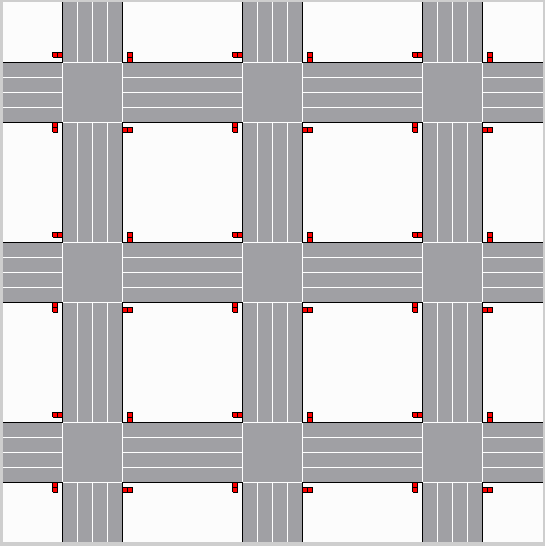
\includegraphics[width=.8\linewidth]{img/intersections.png}
  \caption{The empty intersection grid with all lights red.}
  \label{fig:intersections}
\end{figure}


% TODO: Maak een note over de bug: eerst een reset doen om random seed te genereren.

\section{Results}\label{sec:results}
% test parameters results
The simulations varied by using different number of cars: 50, 100 and 200,
resembling different traffic loads.
The different switch times used were: 2, 4, 8, 16 and 32.
These were chosen since they were either a $\frac{1}{4}$, $\frac{1}{2}$, 1, 2 or 4 times the length of the lanes (8).
For graphing purposes, each algorithm was simulated for 500 simulation steps.
To get consistent results, the random generators are seeded with the same seed for each run.

% TODO: voeg de afbeeldingen in.



\section{Evaluation}\label{sec:eval}

% TODO: evalution and discussion of the results

\subsubsection*{Patterns}

% TODO: describe the pattern emerging with two sided, long switch time

\section{Conclusion}\label{sec:conclusion}

% TODO: write conclusion

\subsection{Future work}

\begin{itemize}
 \item Setting chance choosing between the left lane or the other independently. Now all is equal %Klaas
 \item Giving cars incentive to drive to a certain destination
 \item Make the amount of cars change over time (rush hour effect)
\end{itemize}


\bibliographystyle{acm}

\bibliography{refs}


\end{document}
